%Umisť na novou stránku
\clearpage
% Změna stylu "číslování" stránek
\pagenumbering{Alph}
% Přidání odkazu do obsahu
\addcontentsline{toc}{chapter}{Přílohy}

\section*{Příloha A}

\begin{figure}[H]
	\centering
	\includegraphics[width=\linewidth,page=1]{prilohy/prilohaA/schema.pdf}
	\caption{Schéma zdroje MoSeZ Rev. B}
	\label{priloha:schema_root}
\end{figure}


\begin{figure}[H]
	\centering
	\includegraphics[width=\linewidth,page=2]{prilohy/prilohaA/schema.pdf}
	\caption{Schéma části \emph{Input} zdroje MoSeZ Rev. B}
	\label{priloha:schema_Input}
\end{figure}
\begin{figure}[H]
	\centering
	\includegraphics[width=\linewidth,page=3]{prilohy/prilohaA/schema.pdf}
	\caption{Schéma části \emph{LMA38010} zdroje MoSeZ Rev. B}
	\label{priloha:schema_LMA38010}
\end{figure}
\begin{figure}[H]
	\centering
	\includegraphics[width=\linewidth,page=4]{prilohy/prilohaA/schema.pdf}
	\caption{Schéma části \emph{LM78M33} zdroje MoSeZ Rev. B}
	\label{priloha:schema_LM78M33}
\end{figure}
\begin{figure}[H]
	\centering
	\includegraphics[width=\linewidth,page=5]{prilohy/prilohaA/schema.pdf}
	\caption{Schéma části \emph{ATSAME51J18} zdroje MoSeZ Rev. B}
	\label{priloha:schema_MCU}
\end{figure}
\begin{figure}[H]
	\centering
	\includegraphics[width=\linewidth,page=6]{prilohy/prilohaA/schema.pdf}
	\caption{Schéma části \emph{Current Output} zdroje MoSeZ Rev. B}
	\label{priloha:schema_CurrentOutput}
\end{figure}
\begin{figure}[H]
	\centering
	\includegraphics[width=\linewidth,page=7]{prilohy/prilohaA/schema.pdf}
	\caption{Schéma části \emph{Can Bus Driver} zdroje MoSeZ Rev. B}
	\label{priloha:schema_CanBusDriver}
\end{figure}
\begin{figure}[H]
	\centering
	\includegraphics[width=\linewidth,page=8]{prilohy/prilohaA/schema.pdf}
	\caption{Schéma části \emph{Interface} zdroje MoSeZ Rev. B}
	\label{priloha:schema_Interface}
\end{figure}

\begin{figure}[H]
	\centering
	\includegraphics[width=\linewidth,page=8]{prilohy/prilohaA/pcb_back.jpg}
	\caption{Zadní část DPS MoSeZ Rev. B}
	\label{priloha:pcb_back}
\end{figure}

\FloatBarrier % Vložit za definici sekce

\section*{Příloha B}
\label{prilohaB}

\begin{figure}[H]
	\centering
	\includegraphics[width=\linewidth]{prilohy/prilohaB/boxes_back.pdf}
	\caption{Zadní část krabiček pro MoSeZ Rev. B}
	\label{priloha:boxes_back}
\end{figure}

\begin{figure}[H]
	\centering
	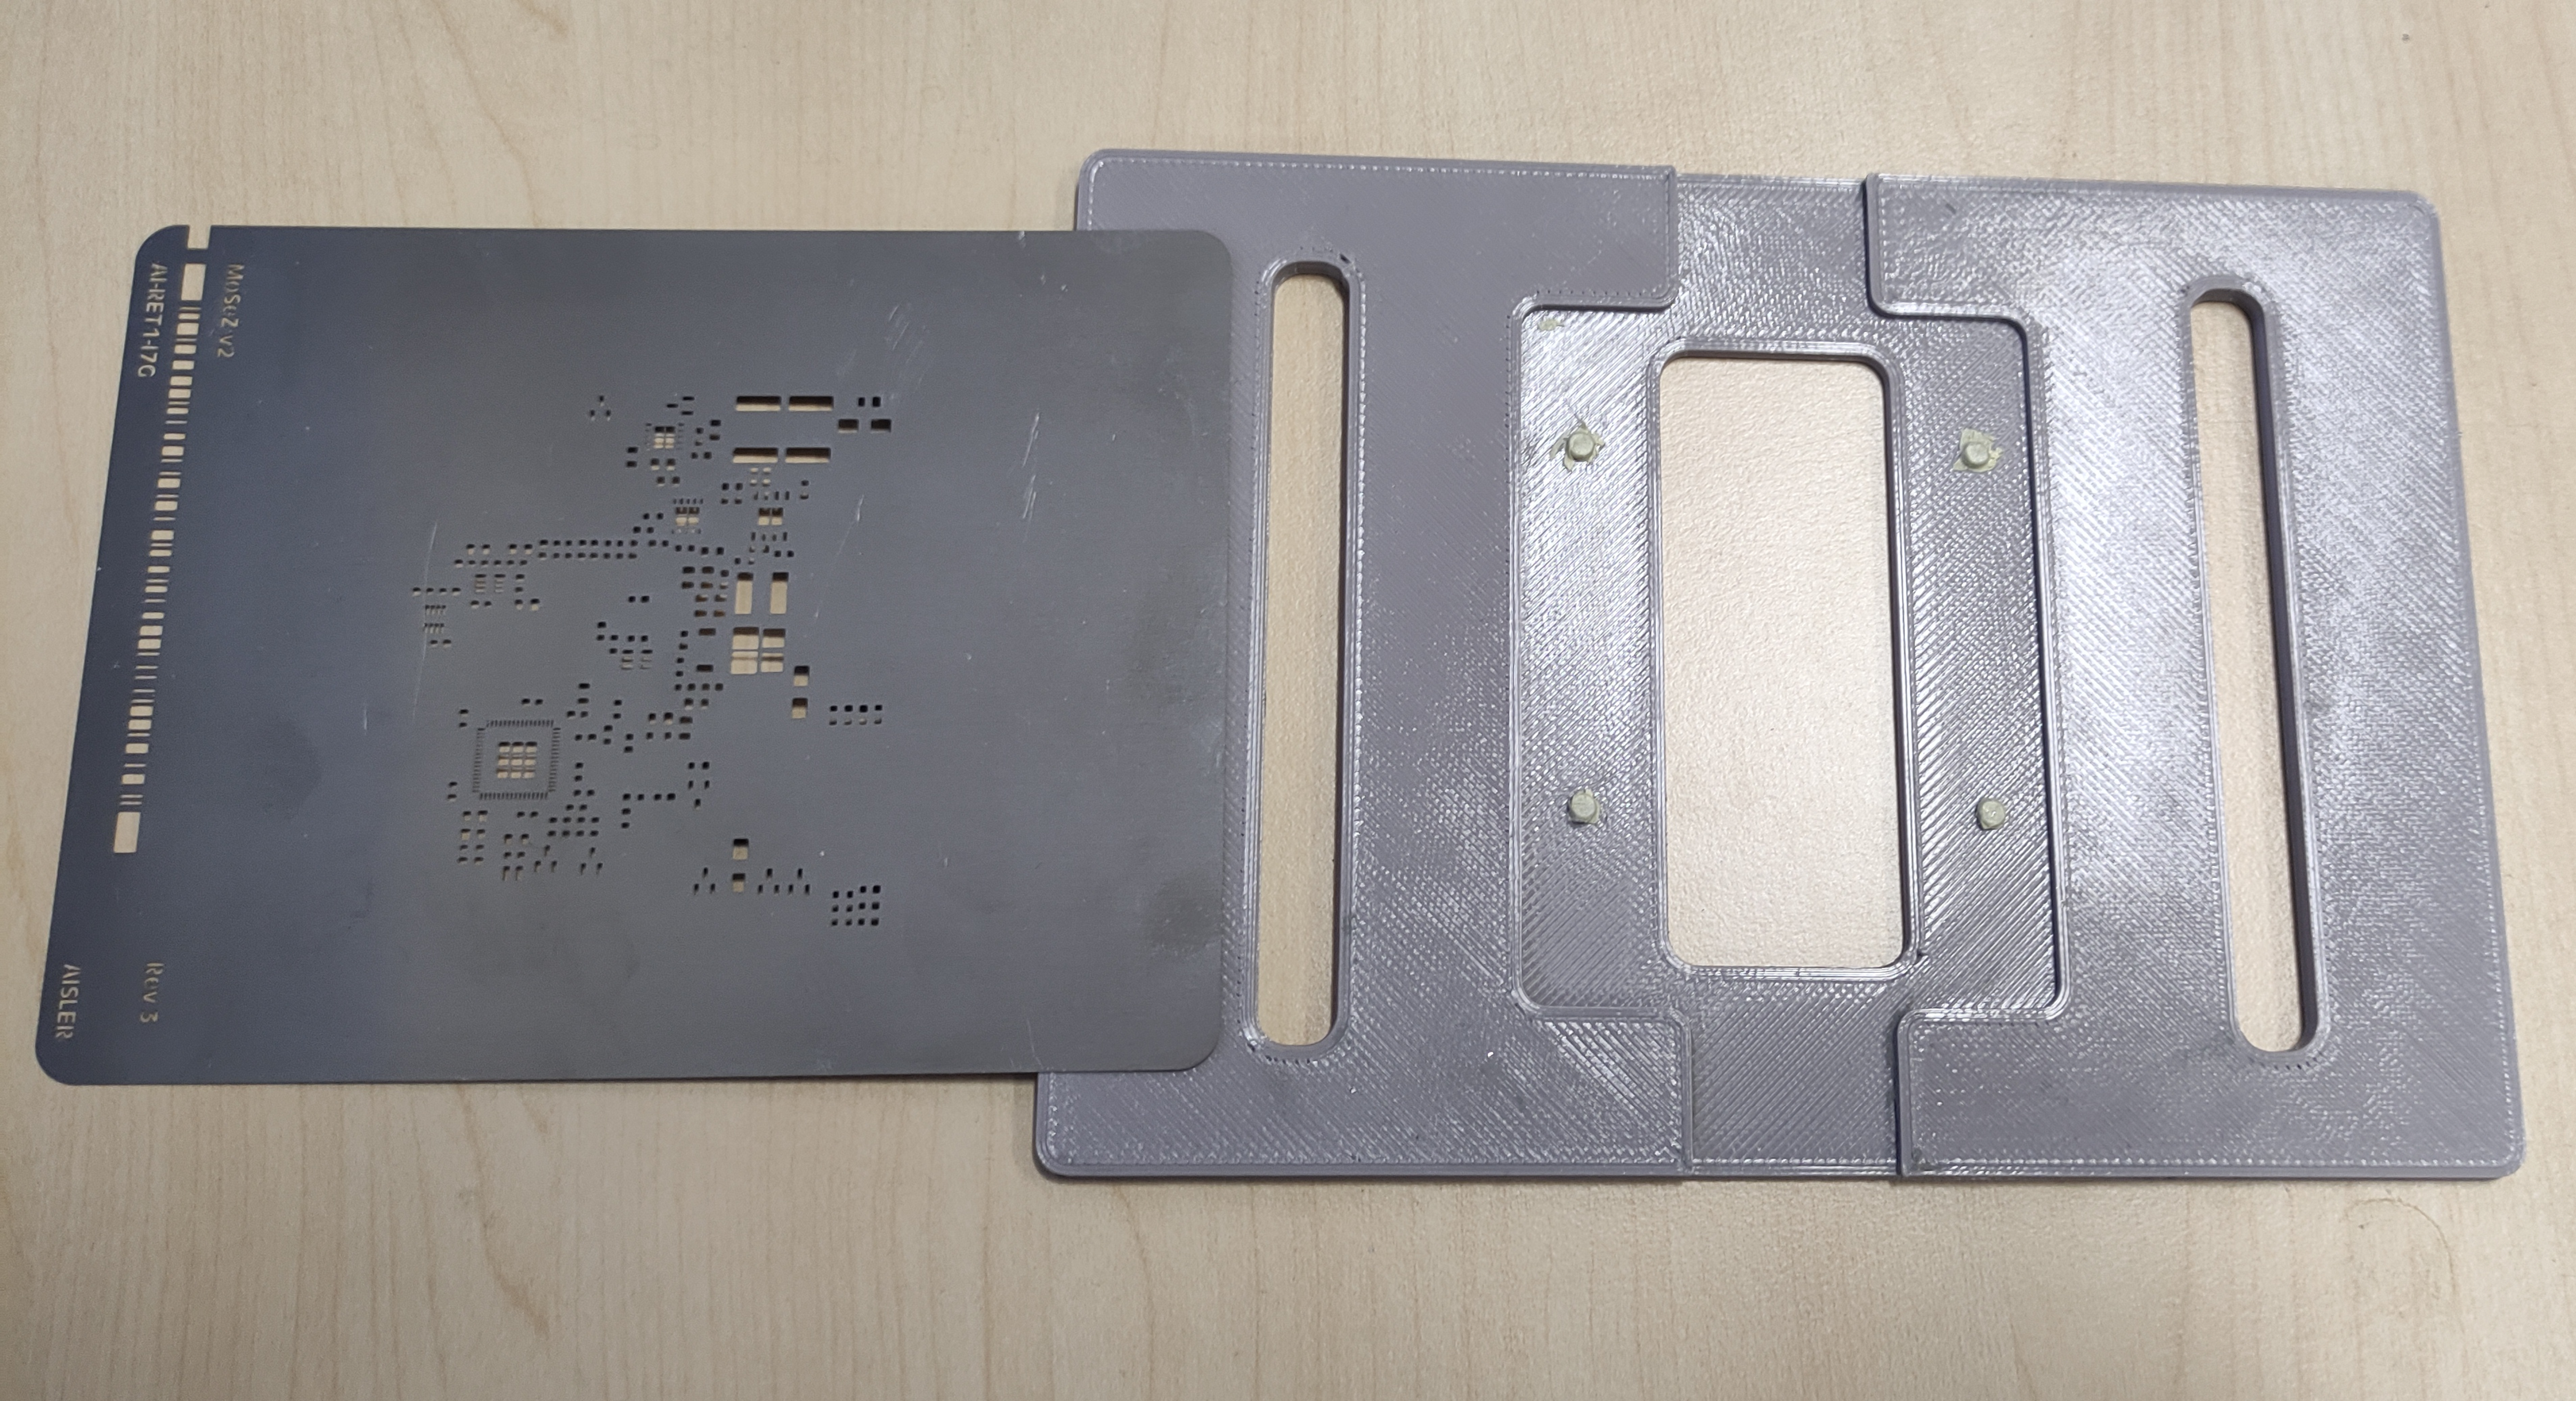
\includegraphics[width=\linewidth]{prilohy/prilohaB/paste_front.pdf}
	\caption{Držák DPS pro aplikaci pájecí pasty na přední stranu DPS}
	\label{priloha:dps_holder_paste}
\end{figure}

\FloatBarrier % Vložit za definici sekce

\section*{Příloha C}

\begin{figure}[H]
	\centering
	\includegraphics[width=\linewidth,page=1]{prilohy/prilohaC/emc_mozes.pdf}  % Replace 10 with last page number
	\caption{Vyzařování rušení na kmitočtech 30 – 1000 MHz desky MoSeZ Rev. B ve standby režimu}
	\label{priloha:mereni_emc_standby}
\end{figure}


\begin{figure}[H]
	\centering
	\includegraphics[width=\linewidth,page=7]{prilohy/prilohaC/emc_mozes.pdf}
	\caption{Vyzařování rušení na kmitočtech 30 – 1000 MHz desky MoSeZ Rev. B se zapnutým výstupem
	a připojeným vstupními a výstupními filtry}
	\label{priloha:mereni_emc_on}
\end{figure}


% Příloha přes celou stranu (pokud má PDF více stran, můžete je zde vyjmenovat pomocí pages={1,2,3} )
%\includepdf[pages={1}]{prilohy/PRILOHA.pdf}

